% Principally, this chapter should describe the work which was undertaken before code was written, hardware built
% or theories worked on. It should show how the project proposal was further refined and clarified, so that the
% Implementation stage could go smoothly rather than by trial and error.

% Throughout this chapter and indeed the whole dissertation, it is essential to demonstrate that a proper 
% professional approach was employed.

% The nature of this chapter will vary greatly from one dissertation to another but, underlining the professional 
% approach, this chapter will very likely include a section headed “Requirements Analysis” and incorporate other 
% references to software engineering techniques.

% The chapter will cite any new programming languages and systems which had to be learnt and will mention 
% complicated theories or algorithms which required understanding.

% It is essential to declare the Starting Point (see Section 7). This states any existing codebase or materials 
% that your project builds on. The text here can commonly be identical to the text in your proposal, but it may 
% enlarge on it or report variations. For instance, the true starting point may have turned out to be different 
% from that declared in the proposal and such discrepancies must be explained.

% ~2500 words

\documentclass[final,rdr32.tex]{subfiles}
\begin{document}

\chapter{Preparation}

This chapter gives a background of current research on various sign-language recognition based models, as well as existing datasets, libraries, and techniques. This forms part of the research conducted prior to writing the implementation code for the project, but will also include further research that has been done in response to challenges encountered during the implementation.

\section{Requirements Analysis}

The task at hand requires a sign language gesture as an input, represented in a suitable format such a video or coordinates. The output should be a prediction of which sign gesture was used as an input.

\begin{figure}[H]
    \begin{center}
        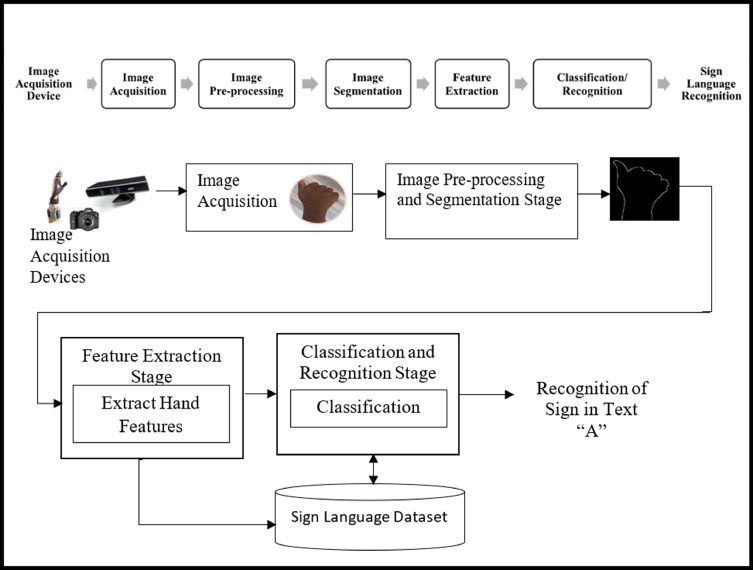
\includegraphics[scale=0.85]{images/task.jpg}
        \caption[caption]{Example pipeline of a sign language recognition model}
    \end{center}
\end{figure}


The project requires the following to be implemented in order to have a working program:

\begin{itemize}
    \item \textbf{Gesture Detection and Tracking}: This is what will determine the shape of the training data and its nature. It consists of identifying and tracking the different body parts present in the given frame, especially hands.
    \item \textbf{Gesture Recognition}: There also needs to be a framework which can accurately predict what gesture has been displayed, from a set of different gestures.
    \item \textbf{Real-time Detection}: The program should allow the gestures to be detected in real-time, giving immediate results.

\end{itemize}

An appropriate dataset is used to perform any form of training or comparison on. Specifically, we target an isolated BSL dataset. However, the nature of sign language in general means that we can expand on different variations of sign language in order to infer how well the model will perform.


\section{Datasets}

\subsection*{BSLDict}

BSLDict is a large dataset of isolated BSL gestures \cite{momeni2020watch}. The data has been obtained from BSL sign aggregation platform \textit{signbsl.com}, with a total of 14k video clips for a vocabulary of 9k labels.

The data provides three main issues:

\begin{itemize}
    \item \textbf{Lack of examples per label: }A lot of the labels have only one or two videos. This is a problem as there is not enough data for testing or to use deep learning for efficient training.
    \item \textbf{Different signs per label: }Many labels contain ambiguous sign gestures. Some of the labels have different ways to represent them and some overlap with other labels as well. This leads to poor accuracy when trying to train on them.
    \item \textbf{Ambiguous number of hands: }Many labels contain sign gestures where it is unknown how many hands are used. Some signs have the hand resting within the frame, which can cause issues for models which depend heavily on the position of both hands.
\end{itemize}

The issue of lacking examples was one reason why DTW was used as an algorithm for this project. As deep learning models require a sufficient amount of training data to be sufficiently accurate, we use a model based on DTW instead as it can retain accuracy with less data.

\begin{figure}[H]
    \begin{center}
        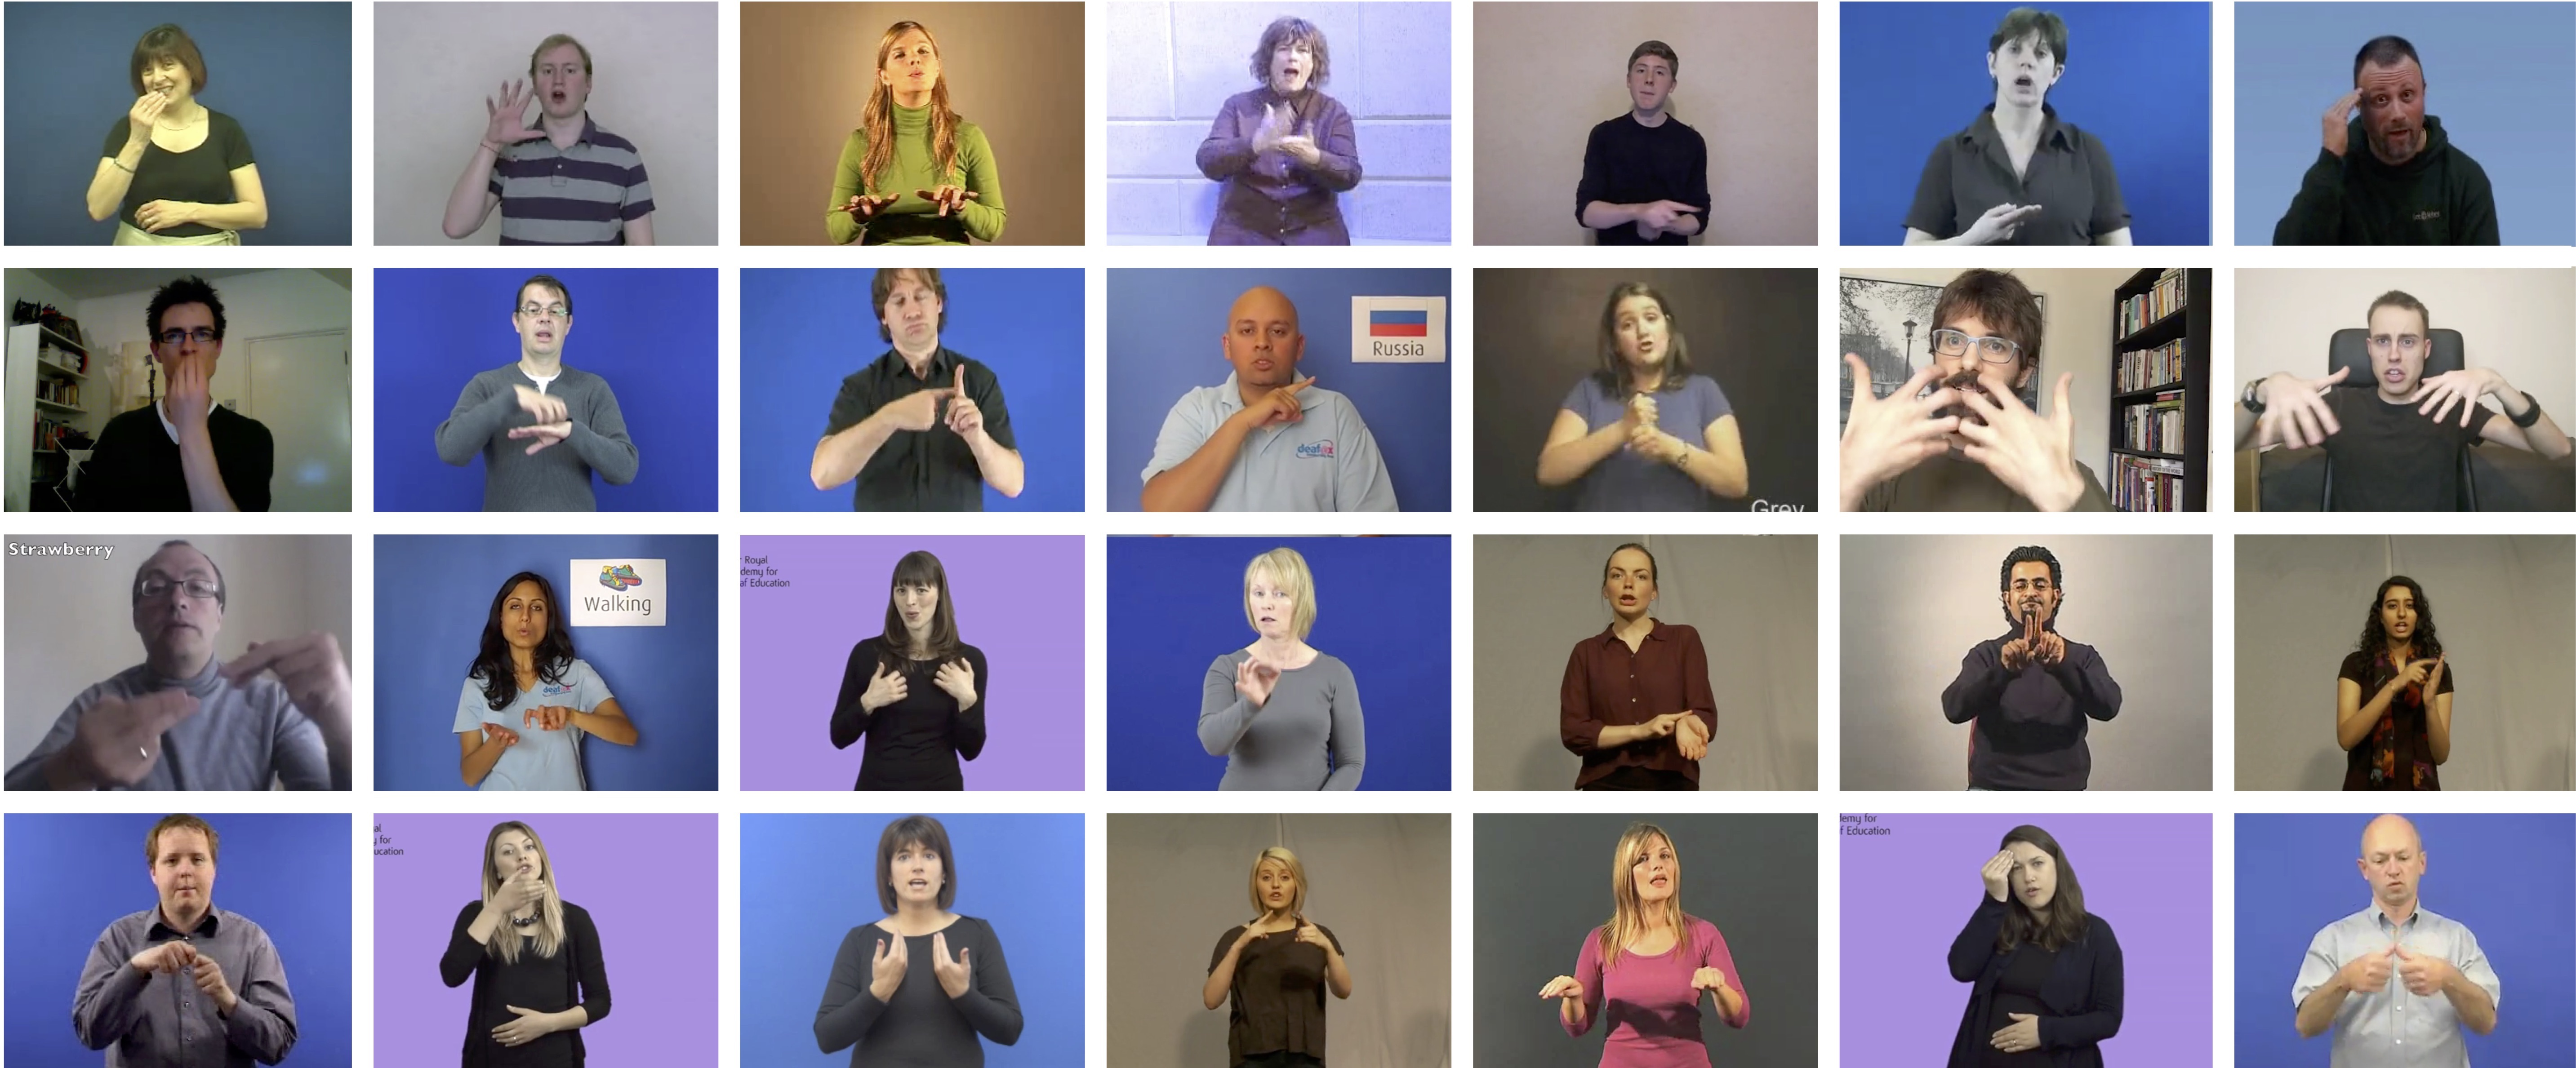
\includegraphics[scale=0.08]{images/BSLDict.jpeg}
        \caption[caption]{Examples from the BSLDict dataset}
    \end{center}
\end{figure}

\subsection*{LSA64}

LSA64 is a sign database for isolated Argentinian Sign Language (LSA) gestures \cite{ronchetti2016lsa64}. It was created to produce a dictionary for LSA and to be used for training automatic sign recognition models. The dataset contains 3200 videos, with 10 signers executing 5 repetitions of 64 different types of signs.

This dataset was used mostly for initial testing purposes given the issues that were encountered with BSLDict. It provides both sufficient data and consistent signs per label.

Signers wore coloured gloves to aid hand recognition and segmentation, as well as wearing dark clothing. This does not affect this project due to the use of Mediapipe to recognise signs.


\begin{figure}[H]
    \begin{center}
        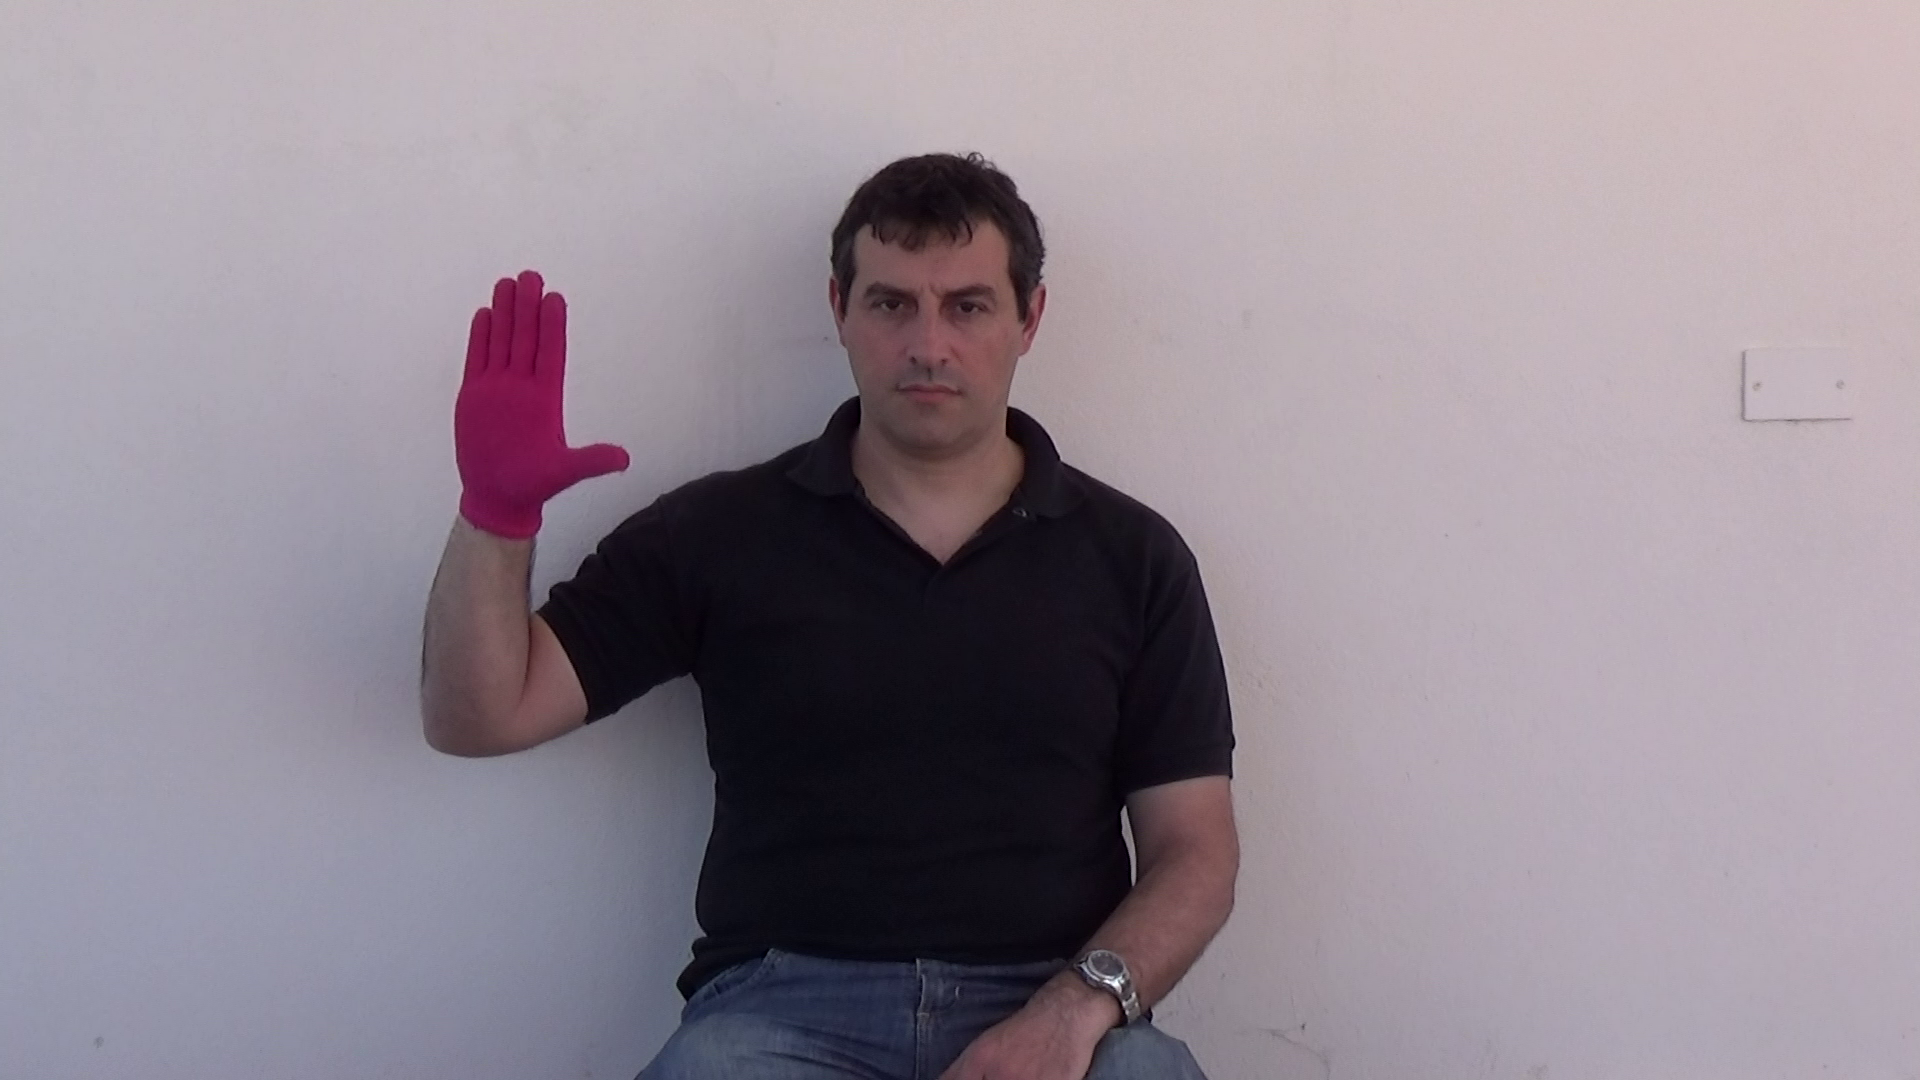
\includegraphics[scale=0.2]{images/LSA64.png}
        \caption[caption]{Snapshot from the LSA64 dataset}
    \end{center}
\end{figure}

\section{Model Selection}

\subsection{Neural Networks}

Studies have been conducted on many different neural network architectures, focused
on mainly on image classification. The best performing networks include 3D Convolutional Neural Networks (3D CNNs), such as I3D, and Recurrent Neural Networks (RNNs), such as Long Short-Term Memory (LSTM) networks. I3D has shown remarkable performance in sign language recognition tasks due to its ability to capture spatiotemporal information from videos. It has been used in various sign language recognition projects, such as recognizing American Sign Language (ASL) gestures, notably on the MS-ASL dataset \cite{joze2018ms}. RNNs, particularly LSTMs, are also commonly used for sign language recognition due to their ability to handle sequential data. These networks have been used in projects aimed at recognizing both isolated gestures \cite{liu2016sign} and continuous sign language sentences \cite{guo2018hierarchical}.

\subsection{Dynamic Time Warping}

Dynamic Time Warping (DTW) is a well-known algorithm for comparing sequences that may have different lengths and may be slightly misaligned. It was first introduced by Sakoe and Chiba in 1978 \cite{sakoe1978dynamic} and has since been widely used in many areas such as speech recognition, pattern recognition, bioinformatics, and finance. The idea to use this algorithm for sign language recogntion was inspired from content in the paper by Huu et al. \cite{huu2014human}.

The basic idea of DTW is to find the optimal alignment between two sequences by warping one of the sequences in the time dimension. The algorithm constructs a distance matrix between the two sequences, where each element represents the distance between a point in the first sequence and a point in the second sequence. The optimal path through this matrix is then found using dynamic programming, which minimizes the total distance between the two sequences.

\begin{figure}[H]
    \begin{center}
        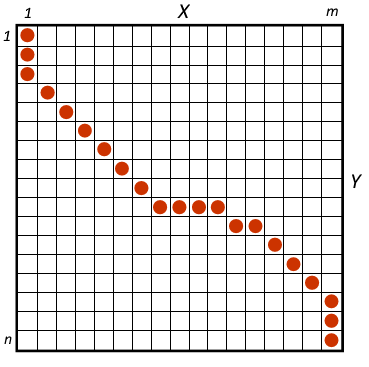
\includegraphics[scale=0.7]{images/DTW.png}
        \caption[caption]{Matrix with warp path}
    \end{center}
\end{figure}


Let $X = {x_1, x_2, ..., x_{m}}$ and $Y = {y_1, y_2, ..., y_{n}}$ be two sequences of length $m$ and $n$, respectively. The algorithm aims to find the optimal path $\pi = {(i_1,j_1),(i_2,j_2),...,(i_k,j_k)}$ that warps one of the sequences (usually the shorter one) to align with the other sequence. The optimal path $\pi$ is the one that minimizes the total distance between the two sequences, which is defined as:

\begin{equation*}
    DTW(X,Y) = \min_{\pi}\sqrt{\sum_{(i,j) \in \pi}(x_i - y_j)^2}
\end{equation*}
where $(i,j)$ represents a point in the distance matrix.

To find the optimal path $\pi$, the DTW algorithm constructs a distance matrix $D$ of size $m \times n$, where each element $D_{i,j}$ represents the distance between $x_i$ and $y_j$. The matrix is initialized with large values such that $D_{i,j} = \infty$ for all $i$ and $j$. The first element is set to $D_{1,1} = (x_1 - y_1)^2$. Then, for each element $D_{i,j}$, the algorithm finds the minimum distance among the three neighboring elements:

\begin{equation*}
    D_{i,j} = (x_i - y_j)^2 + \min(D_{i-1,j}, D_{i,j-1}, D_{i-1,j-1})
\end{equation*}

The path through the distance matrix that corresponds to the optimal path $\pi$ is then found by backtracking from the bottom-right corner of the matrix to the top-left corner, following the minimum distance at each step. The resulting path is the optimal path $\pi$, which can be used to align the two sequences. The time and space complexity of the algorithm are in the quadratic order. In the distance matrix, each cell is filled in exactly once, with each being filled in constant time. That leads to a time and space of complexity of $O(m \times n)$.

Algorithm 1 is a simple implementation of the DTW algorithm in pseudocode.
\begin{algorithm}
    \caption{Simple DTW algorithm}
    \SetKwFunction{isOddNumber}{isOddNumber}
    \SetKwInOut{KwIn}{Input}
    \SetKwInOut{KwOut}{Output}

    \KwIn{X: array $[x_1, x_2, \dots, x_m]$, Y: array $[y_1, y_2, \dots, y_n]$}
    \KwOut{Distance: float}

    $dp = \text{matrix of size } m+1 \times n+1$

    \For{$i \leftarrow 1$ \KwTo $m$}{
        \For{$j \leftarrow 1$ \KwTo $n$}{
            $dp[i,j] = \inf$
        }
    }
    $dp[0,0] = 0$

    \For{$i \leftarrow 1$ \KwTo $m$}{
        \For{$j \leftarrow 1$ \KwTo $n$}{
            $cost = abs(X[i-1] - Y[J])$
            $dp[i,j] = cost + min(dp[i-1,j],
                dp[i, j-1],
                dp[i-1, j-1])$
        }
    }

    \KwRet{$dp[m,n]$}
\end{algorithm}

DTW has been shown to be an effective algorithm for comparing sequences in many applications, but it has some limitations. One of the main limitations is its computational complexity, which is quadratic in the length of the sequences. This can be a problem for very long sequences or for applications that require real-time processing. In recent years, there have been many extensions and variations of DTW that aim to overcome some of these limitations \cite{ratanamahatana2004everything}.

\subsection{Feature Extraction}

Feature extraction is a crucial step in sign language recognition systems as it enables the conversion of raw video data into meaningful and informative representations that can be used for classification purposes. In this section, we discuss the feature extraction process used in our sign language recognition project, which involves the extraction of hand and body pose landmarks and the calculation of hand angles and relative distance features.

The project employed Mediapipe Holistic, an open-source library developed by Google, to extract landmarks from the hand and body poses in the sign language videos. This library provides a robust and accurate solution for the detection of body and hand keypoints, including wrist, elbow, shoulder, and finger joints. Specifically, we used the pre-trained Holistic model, which uses a deep neural network to detect the keypoints and estimate their positions in real-time. More details about Mediapipe are described in both Section \ref{sec:mediapipe-holistic} and Section \ref{sec:mediapipe}.

From the extracted landmarks, angles between each of the 21 hand landmarks were calculated for each hand. This resulted in 441 angles, which captured the intricate hand movements and positions that are characteristic of sign language gestures. These angles were calculated using the law of cosines and were normalized to ensure consistency across different signers and videos.

In addition to hand angles, the relative distance between the wrist and shoulder landmarks was also calculated for each hand. This feature provides information about the arm extension, which is a critical aspect of sign language gesture recognition. The distance feature was calculated as the Euclidean distance between the wrist and shoulder landmarks and was also normalized to ensure consistency.

These methods were used instead of relying on the raw landmark data as distance and positioning greatly affect the accuracy of the results. Angles and relative distances are less sensitive to these factors, thus allowing the model to be accurate even if users are positioned differently or are further away.

\subsection{Alternative Data-Capturing Devices}

Aside from an image feed, there are alternative ways to capture data about hand and body positioning. One sign language recognition paper \cite{chuan2014american} used the Leap Motion controller \footnote{http://www.leapmotion.com}, which reports data in a similar format to Mediapipe. There are also similar studies which have been done using other devices, such as the Microsoft Kinect \cite{lang2012sign}, and the Cyberglove \cite{wang2006american}. The technology can provide more reliable data than images, due to using sensors rather than machine-learning to estimate positions. However, it is sufficient to demonstrate that the model works on a specific format of data, rather than be limited by the device capturing the data. Further work can be undertaken to obtain more accurate results using 3D sensors instead. Moreover, the cost of purchasing such devices is unsuitable for the purpose of a Part II project.

\section{Tools and Libraries}

\subsection*{Python}

Python is a popular high-level programming language that is widely used in scientific computing, data analysis, and machine learning applications. Python was chosen as the main language for this project for the following reasons:

Python has a large and active community of developers, which has contributed to a vast ecosystem of libraries and frameworks that can be used for machine learning and computer vision applications. Some of the popular libraries include NumPy, Pandas, Matplotlib, OpenCV, and Scikit-learn. These libraries provide a range of functionalities, such as data manipulation, visualization, and model development, which can significantly simplify and speed up the development of the project.

Moreover, Python is known for its simplicity and ease of use, making it an ideal language for rapid prototyping and experimentation. The syntax of Python is straightforward and easy to learn, making it an excellent choice for beginners who are new to programming. Additionally, Python's rich standard library provides a wide range of built-in functions and modules that can be used to perform various tasks, such as file I/O, networking, and regular expressions.


\subsection{Visual Studio Code}

Visual Studio Code (VSCode) is a popular and versatile code editor that is widely used for software development, including for Python-based projects. I chose this editor for the following reasons:

VSCode has excellent support for Python programming. It comes with a wide range of built-in features and extensions that facilitate Python development, including code highlighting, linting, debugging, and auto-completion. Additionally, VSCode has a rich and active extension marketplace, where users can access and install a wide range of third-party extensions that enhance its capabilities for Python development.

VSCode provides an intuitive and user-friendly interface that makes it easy to navigate and manage the project code. The built-in file explorer allows for quick navigation through project files and directories, while the integrated terminal provides a convenient way to execute commands and scripts directly within the editor, without needing an external terminal.

Another advantage of VSCode is its support for Git, a version control system that is commonly used in software development projects. With VSCode, we can easily integrate Git into our project workflow, allowing us to manage and track changes to the codebase, collaborate with other developers, and maintain project versions, all done in a very user-friendly environment.

Note that Github Copilot, an AI-powered auto-completion tool, has been used partly in this project while writing the code. This mostly involves autocompleting similar code and finishing standard code fragments required for running the program.

\subsection{OpenCV}

OpenCV (Open Source Computer Vision Library) is an open-source computer vision and machine learning library that provides a wide range of functions for image and video processing, object detection, feature extraction, and more. OpenCV was chosen for the following reasons:

OpenCV supports various programming languages, including Python, C++, and Java, making it a versatile library that can be used in different environments and applications. The project is implemented in Python, and OpenCV provides an intuitive and easy-to-use Python interface that simplifies the development process and speeds up the implementation of the sign language recognition model.

It also has built-in support for hardware acceleration, which can be useful given that the project requires real-time performance as a requirement for the success criteria.

Finally, it is one of the most popular libraries for this purpose, being used by a lot of projects in the field of computer vision. It is well documented and has a lot of support available on its website.

\subsection{Mediapipe-Holistic}
\label{sec:mediapipe-holistic}

Mediapipe Holistic is an open-source library developed by Google that provides a suite of real-time, multi-person pose estimation and tracking solutions. It uses machine learning models to detect and track multiple key points on the human body, including facial landmarks, hand landmarks, and body pose, which can be used for a wide range of applications, including sign language recognition. In this section, we discuss why Mediapipe Holistic is suitable for this project.

Mediapipe Holistic provides a simple and easy-to-use API that abstracts away the complexity of training and deploying machine learning models for pose estimation and tracking. It comes with pre-trained models that can accurately detect and track facial landmarks, hand landmarks, and body pose, which significantly reduces the development time and cost of building a detection model from scratch.

The model is also designed for real-time performance, which is crucial for this project. It provides efficient algorithms that can process video streams in real-time and accurately track multiple body parts simultaneously, which is essential for detecting and recognizing sign language gestures in real-world scenarios.

Additionally, Mediapipe Holistic is an open-source library, which means that it is free to use, distribute, and modify. This open-source nature provides flexibility and enables us to customize and extend the library to suit the specific requirements of the recognition project.

\subsection{dtw-python}

The \verb|dtw-python| library is a Python implementation of the DTW algorithm, which provides a set of functions for computing the DTW distance between two time series data sequences. The library provides an efficient implementation of the DTW algorithm that can handle sequences of different lengths and allows for the customization of the distance function used to compute the DTW distance.

\subsection{FastDTW}
\label{sec:prepfastdtw}

FastDTW is a variant of the DTW algorithm that trades accuracy for faster computation times \cite{salvador2007toward}. It works by reducing the number of elements that need to be computed in the distance matrix, resulting in a smaller memory footprint and faster computation times.

The FastDTW algorithm consists of three main steps: a coarsening step, a projection step, and a refinement step.

The \verb|fastdtw| library in Python provides an implementation of the FastDTW algorithm, as well as other variants of the DTW algorithm. It is useful for this project given that there will be real-time detection involved, so a faster algorithm would speed up the predictions.

\subsection{Git and Github}

Git was used for version control as this is the system that I am most comfortable with using and familiar with. The repository is hosted on Github and changes were pushed regularly. A copy of this dissertation is also available on Github.



\end{document}